\outline{1}{Chapter 4}
\chapter{Compensation and Restitution of Post-Stroke Movement Patterns}
\label{cha:armeospring}



\outline{2}{Introduction}
\section{Introduction}



\outline{2}{Methods}
\section{Methods}

\subsection{Data Collection}

\textbf{Participants.} 
We recruited 11 young (age 23 $\pm$ 2) healthy subjects (7 males) as the control group.
We recruited 53 post-stroke individuals with gender and affected side balanced, shown in table \ref{tab:demog}. 
Participants receive conventional rehabilitation besides robot-aided rehabilitation.

\begin{table}[b]
	\begin{tabular}{c c c c c c c c}
		\hline
		Group & No. & Age & Affected Side & Gender & FM(0-66) & Post Stroke Days & No. of Tests\\
		\hline
		Stroke & 53 & 59$\pm$14 & 29L, 24R & 19F, 30M & 25$\pm$9 to 39$\pm$ 14 & 56$\pm$21 & 80 in 4 weeks \\ 
		Control & 11 & 23$\pm$2 & - & 4F, 7M & - & - & 20 in 1 weeks \\
		\hline
	\end{tabular}
	\caption{Participants information}
	\label{tab:demog}
\end{table}

\textbf{Device.}
Our robot-aided rehabilitation uses ArmeoSpring exoskeleton \cite{} for therapy training. 
Shown in figure \ref{fig:armeo}, the exoskeleton has 7 degrees of freedom, summarized in table \ref{tab:devicedof}. 
It is attached to the arm by two or three velcro straps. 
The exoskeleton has two springs equipped, at the upper arm and forearm respectively. 
The springs can be adjusted to compensate the gravity force of the arm. 
Lengths of the exoskeleton are adjustable, as well as the strength of springs. 
There are no motors at any joints, the user has to move actively to control the exoskeleton. 
The user's trunk is mildly constrained by the velcro strap at the upper arm.  

\begin{figure}
	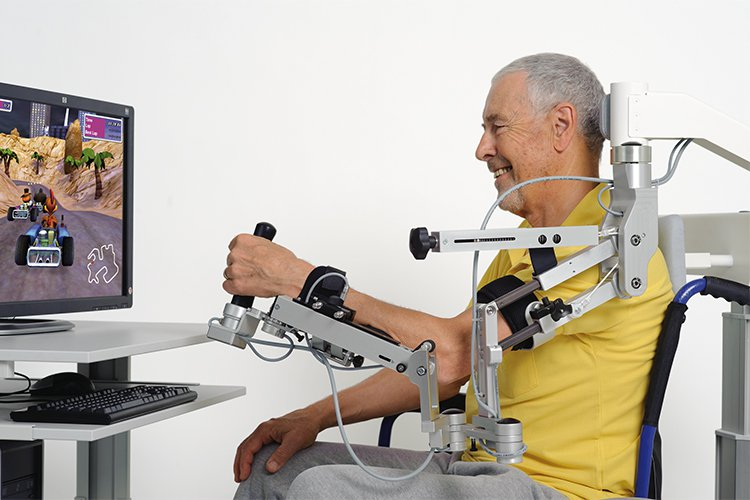
\includegraphics[width=0.5\textwidth]{armeo.jpg}
	\centering
	\caption{ArmeoSpring exoskeleton}
	\label{fig:armeo}
\end{figure}

\begin{table}
	\begin{tabular}{c c c c}
		\hline
		Joint No. & Joint Name & Anatomical Counterpart & Direction \\
		\hline
		1(1) & Inner Shoulder Angle & Shoulder Horizontal Ab-/Adduction & Left/Right \\
		1(2) & Outer Shoulder Angle & Shoulder Horizontal Ab-/Adduction & Left/Right \\
		2 & Upper Arm Angle & Shoulder Flex-/Extension & Up/Down \\
		3 & Elbow Angle & - & Left/Right \\
		4 & Forearm Angle & - & Up/Down \\
		5 & Pro-/Supination Angle & Pro-/Supination & - \\ 
		6 & Flex-/Extension Angle & Wrist Flex-/Extension & - \\
		\hline
	\end{tabular}
	\caption{Degrees of freedom of ArmeoSpring exoskeleton.}
	\label{tab:devicedof}
\end{table}

The device records all joint angles (that is, the joints of the exoskeleton), and calculates the end effector location through a forward kinematics model of the exoskeleton. 
The end effector location then is used to control a cursor on a screen, often displayed vertically in front of the user. 
All joint angles and end effector locations are recorded.

\textbf{Training and Test.}
Participants in the control group receive two training sessions (morning and afternoon) for five consecutive days in a week.
Post-stroke participants receive the same amount of training per day every weekday for 4 consecutive weeks.

One training session consists of several games, each lasts at most 3 minutes (with the exception of the ladybug pointing test mentioned below); after a certain game, the user is often presented with performance feedbacks of that game. 
One training session typically lasts about 20 minutes for young healthy adults.

A ladybug pointing test is scheduled at the beginning and the end of each training session. 
In this test, the user tries to catch ladybugs that appear one by one pseudo randomly on a vertical screen in front of the user. 
The sequence of locations that ladybugs appear are fixed, although within a test they seem random.
The game is two-dimensional; the movement along the dimension perpendicular to the screen is ignored. 
To catch the ladybug, the user moves the cursor to its location. 
The user has limited time to catch the ladybug.
After a ladybug is caught, or time limit is reached, the ladybug disappears and the next ladybug appears somewhere else. 

\subsection{Data Analysis}

\textbf{Preprocessing.}
We filter the data with a second order Butterworth filter with a cutoff frequency of 5 Hz.
We define a trial as the movements between two consecutive ladybugs.
A trial is considered successful if it starts from previously caught target and leads to the catching of next target.

\textbf{Task Space Performance.}
We characterize task space performance via number of peaks in the velocity profile \cite{}.
For participants in the control group, we model the number of peaks ($ p $) with an exponential model

\begin{equation}
p = a e^{-b t} + c
\end{equation}

where $ t $ is test number, $ b $ is learning rate.

For participants in the stroke group, we assume that two components are necessary to model the number of peaks

\begin{equation}
p = a_1 e^{-b_1 t} + a_2 e^{-b_2 t} + c
\end{equation}

\textbf{Joint Space Variability.}
We measure joint space variability approximately by 


\outline{2}{Results}
\section{Results}



\outline{2}{Discussion}
\section{Discussion}



